\section{Rezultatele modelului cu re'tele neuronale}

\subsection{Metodologia de lucru}
\paragraph{}
Am folosit acelea'si date ca 'si 'in capitolul 9, 'imp;ar'tite 'in 85\% date de antrenare, 'si 15\% date de testare. La fel ca 'inainte, am aplicat aceea'si normalizare min-max asupra lor 'inainte de a 'incepe antrenarea re'telei.
\par
Re'teaua a fost antrenat;a folosind algoritmul Levenberg-Marquardt de backpropagare, cu un strat ascuns de 10 perceptroni 'si un num;ar maxim de 1000 de epoci. Arhitectura re'telei poate fi observat;a 'in figura 10.1.
\begin{figure}[!htbp]
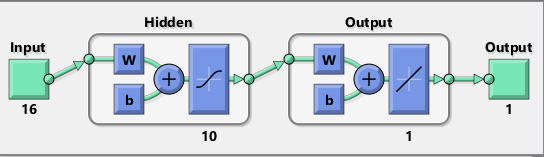
\includegraphics[width=\textwidth]{nnarch}
\caption {Arhitectura re'telei neuronale propuse}
\end{figure}
\subsection{Rezultatele evalu;arii re'telei}
\paragraph{}
Simularea peste cele 18 puncte de test au oferit urm;atoarele rezultate: 
\begin{itemize}
\item O eroare RMSE de 0.227
\item O eroare MMRE de 0.146
\item O estimare PRED(25) de 0.83
\end{itemize}
\par
\begin{figure}[!htbp]
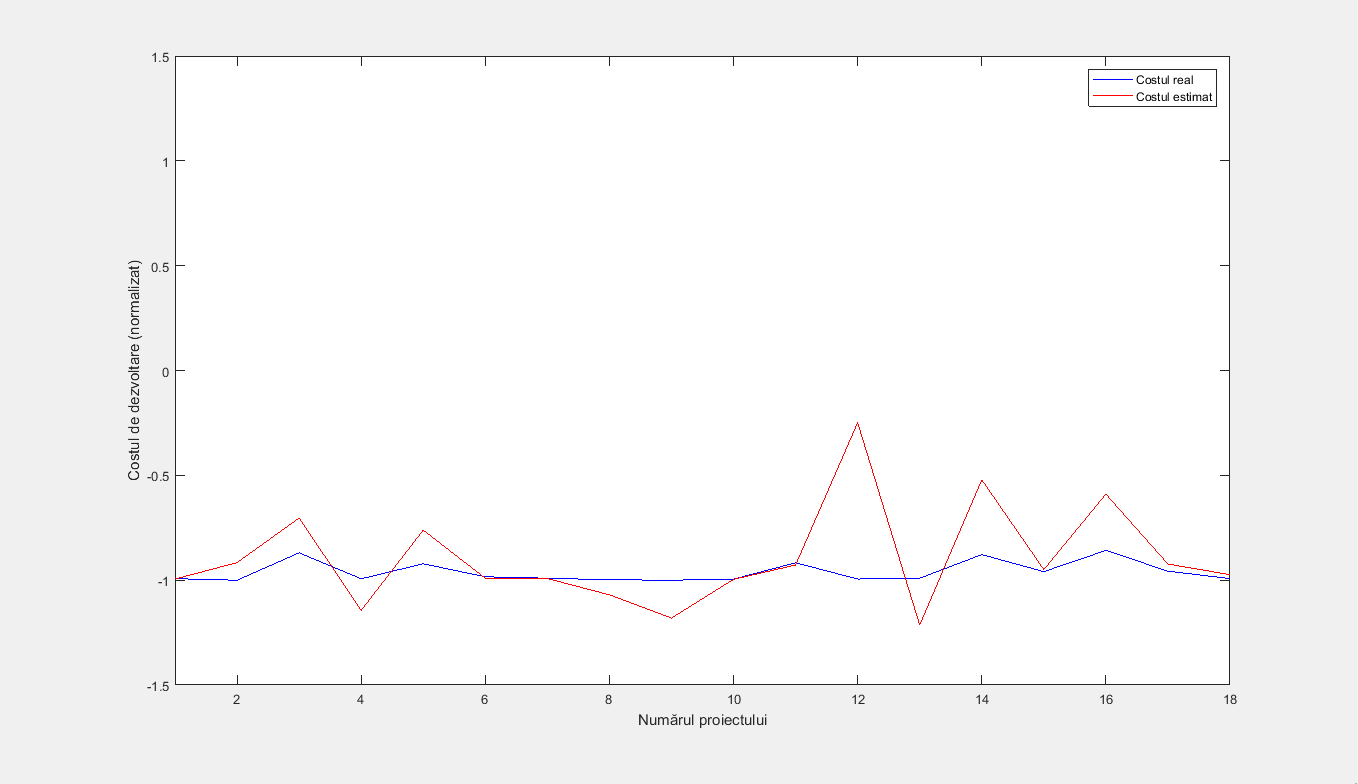
\includegraphics[width=\textwidth]{nntestoutput}
\caption{Rezultatele evalu;arii datelor de test folosind re'teaua neuronal;a propus;a}
\end{figure}
\par
Figura 10.2 ne ofer;a o viziune asupra felului 'in care re'teaua construie'ste predic'tiile peste datele de test. Putem observa c;a unele puncte sunt prezise cu o eroare semnificativ;a, lucru par'tial datorat unui set de date de antrenare restr'ans.